% 
% exemplo genérico de uso da classe iiufrgs.cls
% $Id: iiufrgs.tex,v 1.1.1.1 2005/01/18 23:54:42 avila Exp $
% 
% This is an example file and is hereby explicitly put in the
% public domain.
% 
\documentclass[cic,tc]{iiufrgs}
% Para usar o modelo, deve-se informar o programa e o tipo de documento.
% Programas :
% * cic       -- Graduação em Ciência da Computação
% * ecp       -- Graduação em Ciência da Computação
% * ppgc      -- Programa de Pós Graduação em Computação
% * pgmigro   -- Programa de Pós Graduação em Microeletrônica
% 
% Tipos de Documento:
% * tc                -- Trabalhos de Conclusão (apenas cic e ecp)
% * diss ou mestrado  -- Dissertações de Mestrado (ppgc e pgmicro)
% * tese ou doutorado -- Teses de Doutorado (ppgc e pgmicro)
% * ti                -- Trabalho Individual (ppgc e pgmicro)
% 
% Outras Opções:
% * english    -- para textos em inglês
% * openright  -- Força início de capítulos em páginas ímpares (padrão da
% biblioteca)
% * oneside    -- Desliga frente-e-verso
% * nominatalocal -- Lê os dados da nominata do arquivo nominatalocal.def


% Use unicode
\usepackage[utf8]{inputenc}   % pacote para acentuação

% Necessário para incluir figuras
\usepackage{graphicx}         % pacote para importar figuras
\graphicspath{ {./figures/} }

\usepackage{times}            % pacote para usar fonte Adobe Times
% \usepackage{palatino}
% \usepackage{mathptmx}       % p/ usar fonte Adobe Times nas fórmula
\usepackage{listings}

\usepackage[alf,abnt-emphasize=bf]{abntex2cite}	% pacote para usar citações abnt

% 
% Informações gerais
% 
\title{Modelando uma aplicação de ondas sísmicas através do paralelismo de tarefas}

\author{de Assis}{Lucas Barros}
% alguns documentos podem ter varios autores:

% orientador e co-orientador são opcionais (não diga isso pra eles :))
\advisor[Prof.~Dr.]{Schnorr}{Lucas Mello}

% a data deve ser a da defesa; se nao especificada, são gerados
% mes e ano correntes
% \date{maio}{2001}

% o local de realização do trabalho pode ser especificado (ex. para TCs)
% com o comando \location:
\location{Porto Alegre}{RS}

% 
% palavras-chave
% iniciar todas com letras minúsculas, exceto no caso de abreviaturas
% 
\keyword{programação paralela}
\keyword{programação baseada em tarefas}
\keyword{Ondes3D}
\keyword{StarPU}

%\settowidth{\seclen}{1.10~}

% 
% inicio do documento
% 
\begin{document}

% folha de rosto
% às vezes é necessário redefinir algum comando logo antes de produzir
% a folha de rosto:
% \renewcommand{\coordname}{Coordenadora do Curso}
\maketitle

% dedicatoria
% \clearpage
% \begin{flushright}
%     \mbox{}\vfill
%     {\sffamily\itshape
%       ``If I have seen farther than others,\\
%       it is because I stood on the shoulders of giants.''\\}
%     --- \textsc{Sir~Isaac Newton}
% \end{flushright}

% agradecimentos
%\chapter*{Agradecimentos}
%Agradeço ao \LaTeX\ por não ter vírus de macro\ldots



% resumo na língua do documento
\begin{abstract}
  A aplicação \textit{Ondes3D} tem como objetivo realizar a simulação da propagação de ondas sísmicas utilizando o método de diferenças finitas.
  Apesar de contar com uma implementação paralela utilizando \textit{OpenMP}, esse paralelismo só é obtido dentro de cada uma das quatro grande etapas do algoritmo utilizado.
  O trabalho aqui apresentado estuda as alterações necessárias para dividir as estruturas utilizadas pelo simulador em blocos, possibilitando
  posteriormente uma implementação em forma de tarefas utilizando a biblioteca \textit{StarPU}, possibilitando um nível de paralelismo superior ao atual.
  Depois de feitas as considerações necessárias para a conversão do modelo atual para o modelo baseado em tarefas, uma implementação é proposta e parcialmente
  elaborada, de maneira a explorar as dificuldades envolvidas no processo e analisar, mesmo que parcialmente, os resultados obtidos.
  Finalmente, a partir desse projeto posto em prática, algumas sugestões de aperfeiçoamento são apresentadas, buscando aproveitar a experiência obtida para
  construir uma versão capaz de explorar ainda mais as diferentes arquiteturas hoje existentes.
\end{abstract}

% resumo na outra língua
% como parametros devem ser passados o titulo e as palavras-chave
% na outra língua, separadas por vírgulas
\begin{englishabstract}{Seismic waves modelling through task-based programming}{Parallel programming. Task-based programming. Ondes3D. StarPU}
  The \textit{Ondes3D} simulator aims to simulate the propagation of seismic waves through the finite differences method. Even though it has a parallel implementation using
  \textit{OpenMP}, this parallelism is only achieved inside each of its four major steps.
  The study presented in this document studies the modifications needed to split the structures used by \textit{Ondes3D} in tiles, which
  allows a task-based implementation using the \textit{StarPU} library in order to achieve a higher level of parallelism.
  From the observations made by studying the needed conversion from the current model to a task-based one, an implementation is proposed and partially executed to explore
  the main obstacles involved in the process and, even if partially, analyse the results obtained.
  Finally, taking in account the developed project, some improvements are suggested in order to use the development experience acquired to construct a version capable of
  exploiting even more the current available architectures.
\end{englishabstract}

% lista de figuras
\listoffigures

% lista de tabelas
\listoftables

% lista de abreviaturas e siglas
% o parametro deve ser a abreviatura mais longa
\begin{listofabbrv}{SPMD}
\item[CPU] Central Process Unit
\item[DAG] Directed Acyclic Graph
\item[GPU] Graphics Processing Unit
\item[HPC] High-Performance Computing
\item[MPI] Message Passing Interface
\end{listofabbrv}

% idem para a lista de símbolos
% \begin{listofsymbols}{$\alpha\beta\pi\omega$}
%     \item[$\sum{\frac{a}{b}}$] Somatório do produtório
%     \item[$\alpha\beta\pi\omega$] Fator de inconstância do resultado
% \end{listofsymbols}

% sumario
\tableofcontents

% aqui comeca o texto propriamente dito

% introducao
\chapter{Introdução}
Uma ferramenta importante para a mitigação dos riscos decorrentes de terremotos é a simulação da propagação de ondas sísmicas \cite{Dupros2010HighperformanceFS}. Esse tipo de aplicação
calcula diferentes grandezas físicas a partir de múltiplas iterações sobre uma discretização do espaço analisado em três dimensões, o que resulta em tempos de execução elevados. Por essa razão,
diversos trabalhos, alguns deles apresentados no capítulo \ref{sec:related}, buscam alternativas para acelerar a sua execução, identificando as operações mais custosas e, frequentemente,
explorando possibilidades de processamento paralelo e distribuído.

A aplicação \textit{Ondes3D} realiza a simulação descrita acima através do método de diferenças finitas e utilizando bibliotecas paralelas para obter tempos de execução menores. O
paralelismo local, aquele cujas linhas de execução compartilham a mesma memória, é obtido utilizando a biblioteca \textit{OpenMP}, repartindo o cálculo das células que discretizam o
domínio do cálculo entre diferentes \textit{threads} executadas paralelamente. Além disso, o protocolo \textit{MPI} pode ser usado para repartir o espaço estudado em diferentes regiões,
sendo cada uma delas fornecida a uma unidade de processamento com seu próprio espaço de endereçamento.

Apesar de empregar técnicas que permitem que vários cálculos simultâneos sejam realizados, o paralelismo alcançado pelo \textit{Ondes3D} existe somente dentro de cada uma de suas
quatro grande etapas, sem a possibilidade de entrelaçar a computação de diferentes estruturas. Dessa maneira, as unidades de processamento que concluirem seus cálculos antes das
demais precisam aguardar ociosamente até que todas tenham finalizado a etapa atual.

O paradigma de programação paralela baseada em tarefas, que consiste em construir pequenos blocos de código que atuam diversas vezes sobre diferentes conjuntos de dados, permite a
obtenção de uma granularidade mais fina, isto é, de uma quantidade maior de tarefas a serem distribuídas entre as unidades de processamento, reduzindo a possibilidade de haver
unidades ociosas e, por consequência, acelerando a execução das aplicações que a usam.

A biblioteca \textit{StarPU} é uma alternativa atual que implementa a programação baseada em tarefas. Em sua implementação, uma tarefa consiste em uma função cuja especificação
inclui, além dos dados utilizados, seus modos de acesso: somente leitura, somente escrita ou leitura e escrita. Ao longo do algoritmo, essas tarefas são submetidas à um escalonador
gerenciado pela biblioteca, que utiliza a ordem de submissão e os modos de acesso descritos por cada uma delas para construir um grafo acíclico direcionado (\textit{Directed Acyclic 
  Graph}, ou \textit{DAG}) representando as dependências existentes entre elas. Esse grafo é utilizado ao longo da execução pela bibliteca para distribuir as tarefas conforme as suas
dependências e os recursos computacionais disponíveis.

Este trabalho tem como objetivo estudar e implementar as alterações necessárias para que o algoritmo da aplicação \textit{Ondes3D} seja executado na forma de tarefas gerenciadas
pela biblioteca \textit{StarPU}, resultando em uma granularidade mais fina e no paralelismo entre etapas graças ao gerenciamento de dependências fornecido pela biblioteca, para
posteriormente avaliar o grau de paralelismo obtido.


\section{Contribuições}

O estudo aqui realizado explora algumas das dificuldades envolvidas na implementação do método de diferenças finitas aplicado à simulação de propagação de ondas, como a necessidade
de alternativas para absorver as ondas quando estas atingem os limites artificiais criados pela discretização do problema, e na elaboração de um algoritmo paralelo capaz de aproveitar
ao máximo as unidades de processamento disponíveis.

A partir do estudo realizado, este trabalho fornece também uma tentativa de implementação do simulador \textit{Ondes3D} utilizando o paradigma de programação baseada em tarefas implementado
pela biblioteca \textit{StarPU}. Apesar da versão implementada atualmente não ser capaz de simular corretamente todos os fenômenos físicos envolvidos na simulação, a estrutura geral, assim como
a definição das tarefas que computam as etapas envolvidas no algoritmo e os dados por elas utilizados foram desenvolvidas e servem de base para uma versão correta eventualmente mais
eficiente que a original.

Finalmente, aproveitando as experiências obtidas no desenvolvimento da versão paralela e no estudo de trabalhos similares, algumas propostas de melhorias são sugeridas para uma
eventual sequência do algoritmo implementado.


\chapter{Trabalhos relacionados}\label{sec:related}

A aplicação \textit{Ondes3D} já foi objeto de estudo de outros trabalhos, frequentemente visando um tempo de execução reduzido mas passando também pela busca de um consumo energético 
inferior. Além disso, outras aplicações também empregaram a programação baseada em tarefas para obter uma aceleração nos cálculos realizados. Alguns desses trabalhos são discutidos abaixo.

Boito et al. \cite{boito} verificaram que mais de $72\%$ do tempo de execução do \textit{Ondes3D} é utilizado em operações de leitura e escrita. Três otimizações diferentes foram
propostas: incialmente, uma camada de \textit{software} foi criada para centralizar as solicitações de entrada e saída da aplicação. Em um segundo momento, os passos de comunicação entre
processos foram substituídos por operações de escrita efetuadas diretamente no sistema de arquivos. A terceira implementação passa a utilizar diversos arquivos de saída, o que permite que
múltiplas operações de escrita aconteçam paralelamente. Apesar dos resultados impressionantes desse trabalho, o estudo aqui proposto não tem como foco as operações de entrada e saída mas
sim a paralelização dos cálculos das equações elastodinâmicas, o que permitiria em um momento futuro a combinação das duas otimizações para alcançar uma aceleração ainda mais significativa.

Tesser et al. \cite{dupros:hal-00797682}, partindo de uma implementação distribuída em que o domínio é dividido em partes menores, perceberam que o tempo de cálculo das equações
depende da região sendo tratada, causando um desbalanceamento de trabalho entre os processadores utilizados. Ao utilizar uma implementação de \textit{MPI} construída sobre um suporte
de execução capaz de realizar um balanceamento dinâmico de tarefas, foi possível reduzir o tempo de execução em $23\%$. O presente estudo não considera a utilização de programação
distribuída, mas a granularidade parametrizável alcançada utilizando o modelo proposto permite uma mitigação dos efeitos de uma distribuição desbalanceada. Quanto maior o número de tarefas
disponível em um dado momento, menores são as chances de existirem unidades de cálculo ociosas.

Castro et al. \cite{CASTRO2016108} utilizaram um processador de baixa potência para propor uma implementação da aplicação \textit{Ondes3D} com um baixo consumo energético. A partir
de uma estratégia de ladrilhamento multi-nível, a versão desenvolvida para o processador \textit{MPPA-256} apresentou uma diminuição de $86\%$ do consumo quando comparada à uma
execução em um processador convencional. No entanto, o consumo energético não é um fator considerado no estudo aqui apresentado.

Nesi et al. \cite{nesi} realizaram três implementações diferentes de uma aplicação de dinâmica de fluídos utilizando programação baseada em tarefas através da biblioteca \textit{StarPU}.
Além de incluir tarefas voltadas para \textit{GPU}s, o traço de execução resultante foi avaliado e refinado utilizando o conjunto de ferramentas \textit{StarVZ}. Através do emprego da técnica de
células fantasma no gerenciamento dos vizinhos, explicada na seção \ref{sec:proposal}, foi possível alcançar uma aceleração de $77$x em relação à versão original da aplicação estudada.

Martínez et al. \cite{victor} propuseram uma implementação utilizando a biblioteca \textit{StarPU}, baseada em tarefas e considerando arquiteturas heterogêneas compostas por
\textit{CPU}s e \textit{GPU}s. De um certo modo essa proposta vai além da pesquisa aqui apresentada, onde não existe uma implementação voltada para \textit{GPU}. No entanto, Martínez et al.
optaram por descartas as interações com as bordas do domínio devido a complexidade introduzida pelo uso delas. A melhor performance foi alcançada utilizando quatro \textit{CPU}s e oito
\textit{GPU}s, uma aceleração de $25$x em relação à versão original utilizando doze \textit{CPU}s.

A Tabela \ref{tbl:related_works} resume as diferenças entre os trabalho desenvolvido e os estudos citados acima. Os projetos desenvolvidos por Nesi et al. e Martínez et al. são
os que mais se assemelham ao aqui desenvolvido, apesar do primeiro tratar de uma aplicação diferente e o segundo ignorar uma parcela da simulação.

\begin{table}[htb!]
    \caption{Trabalhos relacionados}
    \begin{center}
        \begin{tabular}{l|l|p{60mm}}
            \textit{Trabalho} & \textit{Aplicação} & \textit{Contexto} \\
            \hline
            \hline
            Boito et al.    & \textit{Ondes3D} & Otimização de operações de entrada e saída \\
            Tesser et al.   & \textit{Ondes3D} & Balanceamento dinâmico de carga             \\
            Martínez et al. & \textit{Ondes3D} & Implementação baseada em tarefas em arquiteturas heterogêneas sem condições de borda             \\
            Castro et al.   & \textit{Ondes3D} & Otimização de consumo energético             \\
            Nesi et al.     & Dinâmica de fluídos & Implementação baseada em tarefas em arquiteturas heterogêneas \\
            Este trabalho   & \textit{Ondes3D} & Implementação baseada em tarefas             \\
            \hline
        \end{tabular}
    \end{center}
    \legend{Fonte: Autor}
    \label{tbl:related_works}
\end{table}

\chapter{Fundamentação teórica}
Para a elaboração desse estudo, primeiramente é necessário compreender o que é a aplicação utilizada. A partir desse conhecimento, é possível tratar do modelo de programação
baseada em tarefas e como ela é implementada na biblioteca \textit{StarPU}. Finalmente, é necessário explicar o método de divisão das estruturas de dados usadas, conhecido como
ladrilhamento ou \textit{tiling}, que permite que as tarefas atuem sobre dados independentes, possibilitando o paralelismo entre elas.

\section{Ondes3D}
A aplicação discretiza o mundo real em diversos tensores tridimensionais, endereçados a partir de suas coordenadas, que representam diferentes grandezas físicas envolvidas
na simulação. Esses tensores são armazenados como atributos de diferentes estruturas de dados, que podem variar de acordo com os dados experimentais utilizados na simulação. No caso
desse trabalho, os dados utilizados são resultado do terremoto de \textit{Chuetsu-Oki}, que atingiu a costa japonesa em 2007. A simulação desse evento é calculada utilizando as
seguintes estruturas de dados:

\begin{itemize}
\item{\textit{STRESS}:} composta por tensores que representam as tensões sofridas em diferentes planos. O tensor $xy$, por exemplo, armazena a tensão sofrida no plano
  $X$ - aquele cuja normal aponta na direção do eixo $X$, isto é, o plano $YZ$ - pelas forças causadas na direção $Y$.
\item{\textit{VELOCITY}:} composta por tensores que representam a decomposição da velocidade da onda nos eixos $X$, $Y$ e $Z$.
\item{\textit{SOURCE}:} composta pelos dados que descrevem a(s) fonte(s) da onda, como seu hipocentro, a longevidade da fonte, sua orientação e sua força.
\item{\textit{MEDIUM}:} composta pelos dados que descrevem o meio por onde a onda se propaga, como sua profundidade.
\item{\textit{ABSORBING\_BOUNDARY\_CONDITION}:} composta por vetores que representam as contribuições das bordas do domínio nos cálculos
  de tensão e velocidade. As contribuições em cada uma dessas grandezas são compostas por nove componentes, representando as influências de
  cada eixo nos três eixos possíveis (no caso da velocidade) e nos três planos possíveis (no caso da tensão). Essas bordas são utilizadas
  para limitar o domínio computacional minimizando a interferência de limites artificiais nos cálculos realizados. \cite{ABCarticle}. 
\end{itemize}

Uma peculiaridade a ser observada nessa aplicação é que, em vez de existir um grande tensor com diversos atributos descrevendo as grandezas físicas que ali atuam, cada grandeza
é armazenada em uma estrutura a parte que possui múltiplos tensores representando as diferentes orientações possíveis. Essa característica trará implicações no gerenciamento de blocos
vizinhos após a operação de ladrilhamento, explicadas em mais detalhes na seção \ref{sec:neighborhood}.

Os cálculos são realizados ao longo de um número pré-determinado de iterações, durante as quais todas as células que compõem o espaço discretizado do problema são atualizadas uma a uma. Esse
padrão de algoritmo, chamado de \textit{stencil}, calcula os valores armazenados em cada célula a partir de valores de células vizinhas, sendo o conceito de vizinhança variável. A Figura
\ref{fig:stencil} ilustra um \textit{stencil} 2D com quatro vizinhos em que o valor da célula ($i$, $j$) envolve os dados das células ($i$, $j-1$), ($i-1$, $j$), ($i+1$, $j$) e ($i$, $j+1$).
Apesar da aplicação estudada usar coordenadas nos eixos X, Y e Z, o mesmo conceito pode ser expandido para o espaço tridimensional.

\begin{figure}[!htb]
    \caption{Representação de um \textit{stencil} 2D com quatro vizinhos}
    \begin{center}
      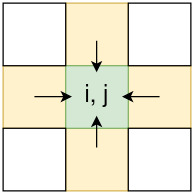
\includegraphics[width=9em]{stencil}
    \end{center}
    \label{fig:stencil}
    \legend{Fonte: Autor}
\end{figure}

As estruturas descritas anteriormente são atualizadas iterativamente passando por quatro grandes etapas, também chamadas de \textit{macro-kernels}. São elas:

\begin{itemize}
\item{\textit{computeSeisMoment}:} etapa em que as fontes da onda são atualizadas.
\item{\textit{computeIntermediates}:} etapa em que as contribuições das bordas do domínio são atualizadas a partir dos tensores de velocidade.
\item{\textit{computeStress}:} etapa em que os tensores de tensão nos diferentes planos são atualizados a partir dos tensores de velocidade e das condições de borda.
\item{\textit{computeVelocity}:} etapa em que os tensores de velocidade são atualizados a partir dos tensores de velocidade e das condições de borda.
\end{itemize}

Com exceção da atualização das fontes da onda, que acontece em um domínio reduzido, os \textit{macro-kernels} descritos acima utilizam a diretiva \textit{omp parallel for}
para obter um paralelismo interno. Já que essas etapas realizam cálculos dentro de um laço triplo, iterando sobre as coordenadas nos eixos $X$, $Y$ e $Z$, a biblioteca \textit{OpenMP},
através da diretiva citada anteriormente, cria \textit{threads} capazes de tratar diferentes coordenadas simultaneamente.

Teoricamente, a partir do momento que a tensão, por exemplo, de uma célula é calculada, já é possível iniciar o cálculo de sua velocidade. No entanto, como a diretiva descrita acima 
é utilizada dentro da função responsável pelo cálculo de tensão de todas as células do domínio, é necessário que todas elas sejam calculadas para que o algoritmo possa iniciar a fase de
cálculo de velocidades. Dessa maneira, apesar da solução atual alcançar uma aceleração graças ao paralelismo introduzido, a quantidade de operações que podem ser executadas simultaneamente
é menor do que seria teoricamente possível. 

\subsection{Condições de borda}

Ao simular a propagação de uma onda, é necessário considerar as reflexões criadas por elas. No entanto, o método de diferenças finitas, utilizado pelo \textit{Ondes3D}, exige que as suas
equações sejam resolvidas em um domínio discretizado restrito. Dessa maneira, ao modelar a propagação de ondas, é necessário utilizar técnicas que permitam absorver as ondas nos limites
do domínio estudado de maneira que suas reflexões não interfiram nos cálculos internos.

Berenger \cite{PML} desenvolveu uma técnica voltada para absorção de ondas eletromagnéticas chamada \textit{Perfectly Matched Layers} (\textit{PML}). Diferentemente
das outras técnicas existentes até então, o emprego de \textit{PML}s permite a construção de uma camada de absorção que teoricamente não produz reflexão alguma independentemente
da frequência e do ângulo de incidência das ondas recebidas. Experimentos realizados na época mostraram que, apesar de uma pequena quantidade de reflexões ter sido detectada,
sua magnitude poderia ser reduzida adequando alguns parâmetros. Além disso, o emprego da técnica de \textit{PML}s permite a utilização de camadas de absorção menos espessas que as
alternativas da época, o que reduz a computação necessária ao simular a propagação de ondas.

Apesar da eficiência do novo técnico desenvolvido, o coeficiente de reflexão das \textit{PML}s só é nulo antes da discretização do domínio e com ondas de incidência não rasante,
isto é, com um angulo de incidência diferente de $90$°, o que torna essa técnica inadequada quando, por exemplo, existem fontes de ondas muito próximas dos limites do domínio. Roden e
Gedney \cite{CPML} propuseram um novo método chamado \textit{Convolutional Perfect Matched Layers}, que utiliza uma convolução recursiva para atenuar a reflexão de ondas de incidência rasante.

A aplicação \textit{Ondes3D} utiliza ambas as técnicas acima descritas em diferentes experimentos. No caso do experimento de \textit{Chuetsu-Oki}, utilizado por esse trabalho, a técnica
empregada é a das \textit{CPML}s.


\section{Paralelismo baseado em tarefas}

O paralelismo baseado em tarefas é um modelo em que se busca descrever trechos de código paralelizáveis na forma de tarefas, que são criadas em tempo de execução pela biblioteca de
paralelismo utilizada. Depois de criar a tarefa, a biblioteca é responsável por executá-la ou adicioná-la a uma fila de tarefas para que ela seja executada em um momento apropriado.
A possibilidade de adiar a execução de uma tarefa é o que torna essa opção interessante ao considerarmos as dependências da aplicação aqui estudada.

\subsection{StarPU}

\textit{StarPU} é uma biblioteca de programação em tarefas para arquiteturas heterogêneas. Ela foi criada visando atender à necessidade da comunidade de \textit{HPC} de
poder computacional \cite{StarPU}, criando uma ferramenta que facilita a criação de tarefas para diferentes arquiteturas e a especificação dos dados utilizados. No caso do estudo aqui
descrito, essa biblioteca é especialmente interessante ao determinar o momento de execução de suas tarefas, já que a escolha desse momento é baseada nas dependências de dados
existentes entre elas.

A utilização de tarefas é composta por dois instantes, sendo o primeiro deles a sua descrição e o segundo a sua inserção, ou submissão, na fila de tarefas. O paralelismo obtido
é o resultado da inserção de diversas instâncias da mesma tarefa atuando sobre dados diferentes e tendo sua ordem de execução determinada pelas dependências entre elas.

A criação de uma tarefa começa pela construção um \textit{kernel}, uma função que implementa a tarefa a ser executada e que deve seguir a seguinte interface:

\begin{verbatim}
void task_name(void *buffers[], void *cl_arg)
\end{verbatim}

Nessa interface, os \textit{buffers} representam os dados que serão gerenciados pela biblioteca levando em conta suas dependências e modos de leitura. Já a estrutura
\textit{cl\_arg} guarda ponteiros de valores externos utilizados pelo \textit{kernel} e são tipicamente valores constantes. O suporte à arquiteturas heterogêneas fornecido pela
biblioteca vem da possibilidade de criação de diversos \textit{kernels} para uma mesma tarefa, sendo cada um deles específico para uma unidade de cálculo distinta.

Com o \textit{kernel} criado, utiliza-se uma estrutura chamada \textit{codelet} para descrever a tarefa. Nessa estrutura é indicada a quantidade de \textit{buffers} utilizados
pela tarefa, seus modos de acesso e o nome dos \textit{kernels} que implementam-na. Voltando ao exemplo da função \textit{computeIntermediates}, um \textit{codelet}
possível é mostrado na Figura \ref{fig:intermediates_cl}.

\begin{figure}[!htb]
    \caption{Definição do \textit{codelet} da função \textit{computeIntermediates}}
    \begin{center}
      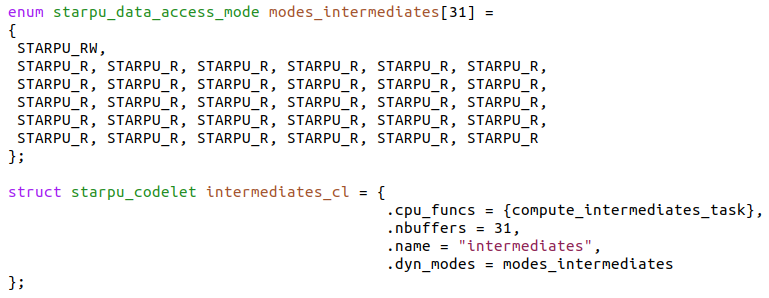
\includegraphics[width=32em]{intermediates_cl}
    \end{center}
    \label{fig:intermediates_cl}
    \legend{Fonte: Autor}
\end{figure}

A biblioteca segue o modelo \textit{STF} (\textit{sequential task flow}), em que uma única \textit{thread} é responsável pelo fluxo principal da aplicação, incluindo a submissão das tarefas,
o que permite que um fluxo paralelo seja facilmente descrito através de um algoritmo sequencial. As tarefas são submetidas sequencialmente e, a partir de sua ordem de submissão e suas dependências,
cria-se um grafo acíclico direcionado que descreve a hierarquia existente entre elas. A partir desse grafo, é possível escalonar as tarefas em tempo de execução de maneira que todas as dependências
sejam respeitadas e o tempo ocioso nas unidades de cálculo seja o menor possível.

A submissão de tarefas é realizada através da função \textit{starpu\_insert\_task}, tendo como parâmetros o \textit{codelet} correspondente, os \textit{buffers} utilizados e
os ponteiros registrados como \textit{cl\_args}. 

\subsection{Matrizes \textit{ladrilhadas}}

Uma estratégia recorrente na programação de alta performance é o ladrilhamento de matrizes - no caso desse estudo, de tensores. Essa técnica consiste, conforme ilustra a Figura \ref{fig:tiled_matrix},
na divisão de uma matriz em sub-matrizes (tipicamente chamadas de blocos) de menor tamanho, indexadas pela sua posição em relação à matriz original.

\begin{figure}[!htb]
    \caption{Decomposição da matriz A em blocos}
    \begin{center}
      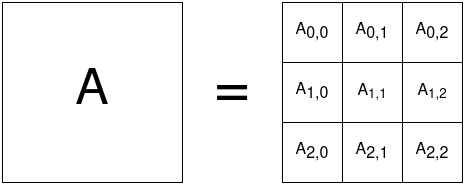
\includegraphics[width=27em]{tiled_matrix}
    \end{center}
    \label{fig:tiled_matrix}
    \legend{Fonte: Autor}
\end{figure}

O ladrilhamento de matrizes exige que os algoritmos sejam re-adequados à sua estrutura, mas em contrapartida oferece numerosas vantagens. Em primeiro lugar, pode-se citar a
otimização dos acessos em memória: ao utilizar um tamanho de bloco suficientemente pequeno, é possível que, durante a execução do cálculo sobre cada um dos blocos, todos os dados
necessários estejam presentes simultaneamente na memória cache. Além disso, utilizando o DAG criado por ferramentas como a biblioteca \textit{StarPU}, é possível executar
simultaneamente tarefas de etapas diferentes, acelerando ainda mais a execução da aplicação.

A Figura \ref{fig:gemm} ilustra o cálculo de multiplicação de matrizes utilizando matrizes ladrilhadas. A versão convencional do algoritmo consiste em acumular a soma dos produtos de
cada linha por cada coluna das matrizes envolvidas. Apesar dos elementos consecutivos de uma mesma linha encontrarem-se tipicamente lado a lado em memória, os saltos realizados nas trocas
de linha podem exigir uma reescrita completa da cache.

\begin{figure}[!htb]
    \caption{Representação do algoritmo de multiplicação de matrizes por blocos}
    \begin{center}
      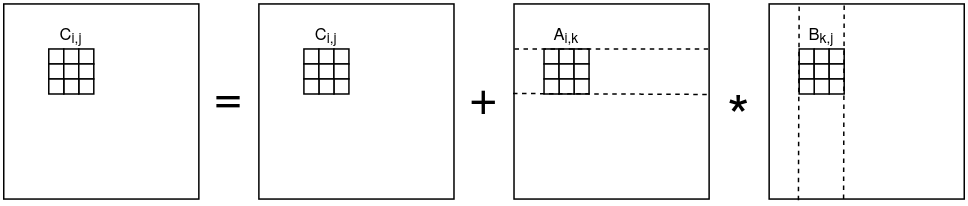
\includegraphics[width=35em]{gemm}
    \end{center}
    \label{fig:gemm}
    \legend{Fonte: Autor}
\end{figure}

A versão ladrilhada é composta por diversas execuções do algoritmo convencional, atuando sobre uma linha (respectivamente, coluna) de blocos de cada vez. Dessa forma, além de otimizar os
acessos de memória ao realizar pequenas multiplicações bloco a bloco, é possível executar o cálculo de $n$ blocos simultaneamente, sendo $n$ o número de blocos que compõem a matriz resultante.
Apesar dos blocos das matrizes $A$ e $B$ serem acessados por diversas tarefas, nenhuma operação de escrita é efetuada sobre eles, o que possibilita que um número qualquer de tarefas acessem-nos
simultaneamente sem gerar incoerências. Os blocos da matriz $C$, onde as escritas são realizadas, são acessados cada um deles por uma única tarefa, possibilitando o paralelismo descrito anteriormente.

\chapter{Projeto e implementação}
Neste capítulo serão apresentadas as alterações necessárias para que a aplicação \textit{Ondes3D} seja paralelizável na forma de tarefas gerenciadas pela biblioteca \textit{StarPU}.
Posteriormente uma descrição da implementação realizada ao longo dessa pesquisa será detalhada.

\section{Proposta}\label{sec:proposal}

Os diversos tensores que representam as grandezas utilizadas nas equações elastodinâmicas do problema deverão ser divididos, de forma parametrizável, em blocos de tamanho igual, que servirão
de entrada para as tarefas implementadas. A Figura \ref{fig:cuboids} ilustra o particionamento realizado pela implementação original, que parte de um arquivo de topologia para discretizar o
plano $XY$ em blocos de profundidade igual à do domínio.

\begin{figure}[!htb]
    \caption{Representação do espaço particionado em nove blocos}
    \begin{center}
      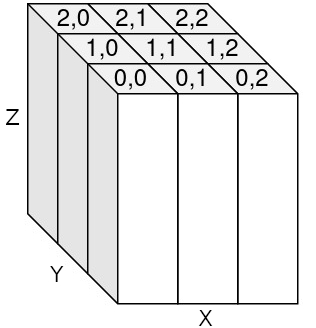
\includegraphics[width=15em]{cuboids}
    \end{center}
    \label{fig:cuboids}
    \legend{Fonte: Autor}
\end{figure}

Em relação ao laço principal de execução, a Figura \ref{fig:main_loop} resume o fluxo da aplicação original. O domínio do problema é dividido em cinco regiões denominadas \textit{imodes},
sendo quatro delas as linhas e colunas externas do domínio e a quinta os elementos internos. Com exceção da etapa \textit{computeSeisMoment}, cada \textit{macro-kernel} é executado cinco
vezes, uma em cada região. Internamente, cada etapa percorre o espaço [$x_{min}$, $x_{max}$][$y_{min}$, $y_{max}$][$z_{min}$, $z_{max}$].

\begin{figure}[!htb]
    \caption{Laço principal da aplicação original}
    \begin{center}
      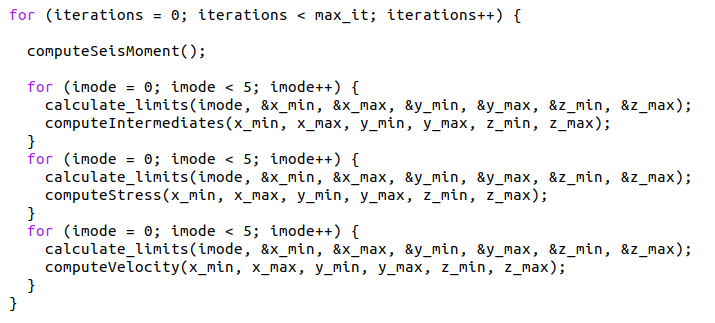
\includegraphics[width=30em]{main_loop}
    \end{center}
    \label{fig:main_loop}
    \legend{Fonte: Autor}
\end{figure}

Na versão aqui proposta, cada etapa será executada tantas vezes quanto houverem blocos. Para isso, será necessário iterar sobre os blocos existentes, criando uma tarefa para atualizar cada bloco
de dados, conforme mostra a Figura \ref{fig:new_main_loop}, dispensando a utilização dos \textit{imodes}. Neste momento vale ressaltar que a inserção das tarefas consiste
simplesmente na criação de uma instância de tarefa com as dependências indicadas e não implica em sua execução imediata. Fica a cargo da biblioteca \textit{StarPU} iniciar a execução
de cada uma das tarefas disponíveis de maneira assíncrona quando as suas dependências assim permitirem. Internamente, cada tarefa percorrerá apenas o espaço determinado pelo bloco a ser
atualizado em vez de uma região completa como na versão original.

Outro ponto a ser ressaltado é o fato de cada tarefa, na verdade, utilizar diversos blocos, já que as grandezas físicas são implementadas em diferentes estruturas. Por exemplo, o cálculo das
tensões efetuado na função \textit{computeStress} necessita não apenas do bloco de índice ($i$, $j$) de cada um dos nove componentes de tensão (em modo de escrita), mas também os blocos de
índice ($i$, $j$) dos três componentes de velocidade, em modo de leitura.

\begin{figure}[!htb]
    \caption{Laço principal da proposta}
    \begin{center}
      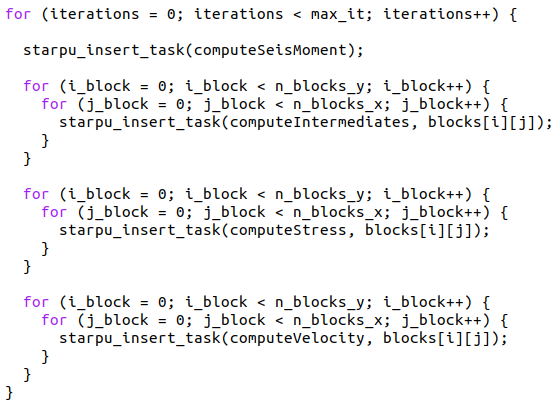
\includegraphics[width=25em]{new_main_loop}
    \end{center}
    \label{fig:new_main_loop}
    \legend{Fonte: Autor}
\end{figure}

A utilização de blocos independentes introduz, no entanto, uma dificuldade nas aplicações do tipo \textit{stencil}: os elementos nas bordas de cada um dos blocos terão como vizinhos
elementos de outros blocos. Uma primeira solução, mais simples e menos eficiente, consiste em não utilizar somente um bloco por tarefa, mas sim cinco - o bloco a ser calculado, em
modo de leitura e escrita, e os seus quatro vizinhos imediatos, em modo de leitura. Essa alternativa, dependendo do contexto em que ela é utilizada, pode representar um custo de memória mais
elevado do que o necessário.

Uma solução mais eficiente é a utilização das chamadas \textit{ghost cells}. Já que é necessário ler apenas as células de uma borda de cada um dos vizinhos, em vez de acessar os quatro
blocos vizinhos completos, compartilha-se apenas as bordas que serão necessárias. A Figura \ref{fig:ghost_cells} mostra um exemplo de células fantasma em um \textit{stencil} 2D,
mas o conceito pode ser expandido para três dimensões.

\begin{figure}[!htb]
    \caption{Representação do uso de células fantasma}
    \begin{center}
      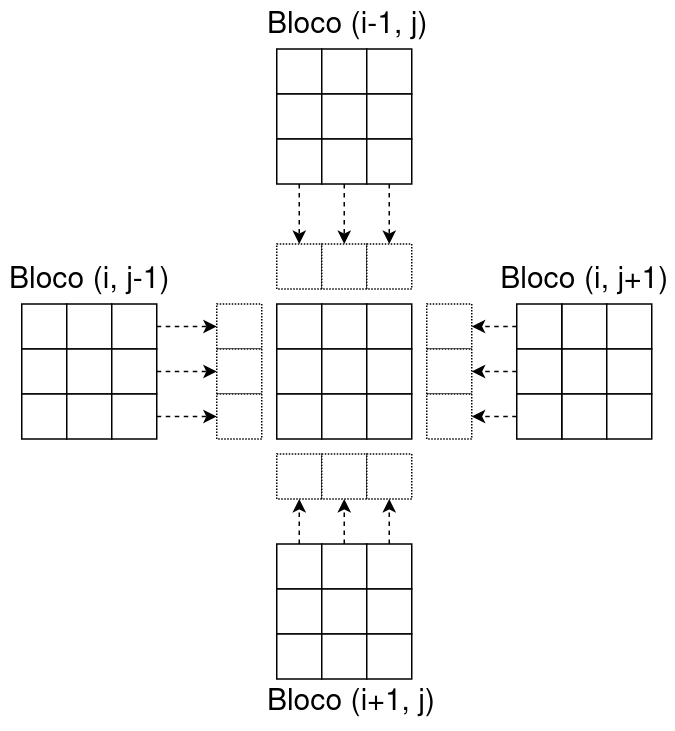
\includegraphics[width=20em]{ghost_cells}
    \end{center}
    \label{fig:ghost_cells}
    \legend{Fonte: Autor}
\end{figure}

\section{Implementação}

A fim de explorar as dificuldades da implementação em forma de tarefas e de analisar o nível de paralelismo alcançável utilizando esse paradigma, uma versão da aplicação \textit{Ondes3D} foi
desenvolvida utilizando a biblioteca \textit{StarPU}. As subseções seguintes detalham o processo de implementação realizado.

\subsection{Inicialização}

A inicialização dos dados na nova versão desenvolvida precisa considerar a necessidade de particioná-los em blocos, o que traz a tona a primeira modificação a ser realizada. A biblioteca
\textit{StarPU} fornece funções que realizam essa operação de ladrilhamento a partir do número de blocos desejado, o que garante um particionamento eficaz e funcional. No entanto, os tensores
utilizados pela versão original são implementados como vetores multidimensionais, o que facilita o acesso aos dados utilizados, e as funções de particionamento da biblioteca \textit{StarPU} exigem
vetores unidimensionais como entrada. Portanto, o primeiro passo para adaptar o algoritmo desenvolvido de maneira a melhor aproveitar as funcionalidades oferecidas pela biblioteca foi a transformação 
de seus vetores multidimensionais em vetores unidimensionais de tamanho equivalente.

Ainda tratando de vetores, a aplicação original realizava um acesso a partir de suas coordenadas, mesmo se elas possuíssem valores negativos. A figura \ref{fig:negative_index} mostra a
técnica utilizada para alcançar esse efeito. Os ponteiros que endereçavam essas estruturas apontavam não para a primeira posição alocada, como normalmente é feito, mas para o n-ésimo elemento,
onde $n$ é a coordenada de valor mais negativo. Devido à complexidade em manter essa implementação utilizando vetores unidimensionais, optou-se por empregar um endereçamento convencional.

\begin{figure}[!htb]
    \caption{Representação de um vetor que permite índices negativos}
    \begin{center}
      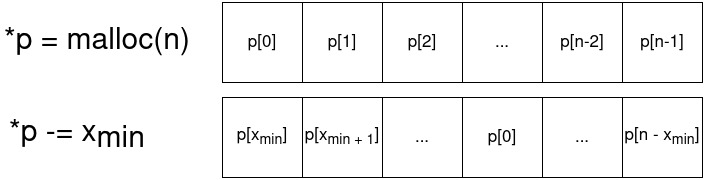
\includegraphics[width=28em]{negative_index}
    \end{center}
    \label{fig:negative_index}
    \legend{Fonte: Autor}
\end{figure}

Devido às mudanças de dimensionalidade e limites dos vetores, o acesso à essas variáveis se torna mais complexo. Para contornar esse problema, foram utilizadas \textit{macros} que calculam
o endereço desejado a partir das dimensões do vetor acessado e das posições solicitadas, detalhadas na seção \ref{sec:tasks}.

\subsubsection{Inicialização das \textit{CPML}}

As \textit{ABSORBING\_BOUNDARY\_CONDITION} não representam o domínio completo do
problema, já que elas tratam unicamente das bordas, onde a propagação da onda deve ser absorvida sem produzir reflexões. Como elas são
responsáveis por registrar contribuições tanto nos tensores de tensão quanto nos de velocidade, ambos construídos com nove componentes,
armazená-las em tensores de tamanho igual ao do domínio exigiria um espaço de memória enorme e esparso, já que elas são calculadas somente
em regiões muito limitadas do domínio.

A fim de não utilizar memória de maneira desnecessária, as contribuições físicas das \textit{CPML}s são registradas em vetores
unidimensionais de tamanho igual ao número de elementos nas mesmas. Um tensor chamado \textit{ipml} armazena, para cada coordenada
do domínio, o índice onde se encontram suas contribuições nos vetores das \textit{ABSORBING\_BOUNDARY\_CONDITION}s. No caso de coordenadas
internas, esse índice tem valor $-1$, indicando que a célula em questão não precisa considerar contribuição alguma. 

Ao dividir o problema em tarefas, no entanto, essas estruturas adicionam novas complexidades. Primeiramente, não é possível aplicar
o particionamento em blocos da mesma maneira nesses vetores, já que eles possuem dimensões reduzidas, iguais ao número de elementos
nas bordas. Além disso, faz-se necessário encontrar uma maneira de, mesmo após particioná-las, associar corretamente as coordenadas das células
aos seus índices no vetor $ipml$.

Outra dificuldade encontrada no particionamento dessas estruturas é mostrada na Figura \ref{fig:ipml}, que ilustra uma matriz de velocidades $v_x$
e um vetor $phiv_x$, que armazena as contribuições das bordas em $v_x$. Considerando que as cores da figura codificam o bloco ao qual cada célula
pertence, pode-se constatar que não é possível particionar os vetores de maneira convencional, pois as contribuições de um
mesmo bloco não são necessariamente sequenciais. Naturalmente, ao considerarmos o espaço tridimensional no qual os cálculos são feitos,
esses fatores se comportam de maneira similar.

\begin{figure}[!htb]
    \caption{Representação de uma matriz de velocidades e um vetor de contribuições das bordas}
    \begin{center}
      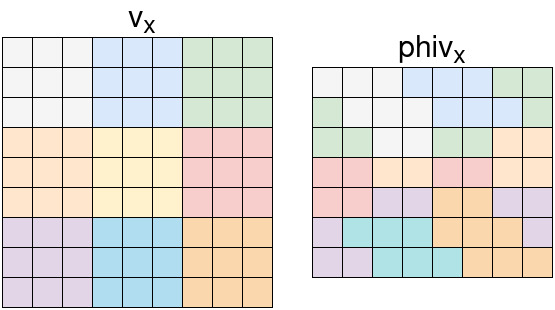
\includegraphics[width=28em]{ipml}
    \end{center}
    \label{fig:ipml}
    \legend{Fonte: Autor}
\end{figure}

Apesar das dificuldades acima apresentadas, é necessário encontrar uma alternativa de particionamento para esses vetores. O \textit{macro-kernel
  computeIntermediates}, por exemplo, acessa as contribuições das bordas em modo de escrita. Portanto, caso
nenhum particionamento seja feito, mesmo que várias tarefas sejam submetidas para tratar diferentes regiões do problema, elas
não poderão ser executadas em paralelo devido à necessidade de escrever em um mesmo vetor. Por esse motivo, é necessário encontrar
uma alternativa de particionamento para esses vetores.

A solução implementada para este estudo começa pela transformação da estrutura de dados das condições de borda, conforme mostra
a Figura \ref{fig:abc}. Os diversos vetores que compunham as contribuições no cálculo de velocidade, por exemplo, foram encapsulados
em uma nova estrutura \textit{phiv\_t} (respectivamente \textit{phit\_t} no caso da tensão), composta por um endereço de base, pelo
tamanho de seus vetores e pelo deslocamento existente entre seus endereços.

\begin{figure}[!htb]
  \caption{À esquerda, parte da implementação da estrutura de condições de borda e, à direita, parte da
  nova implementação proposta.}
    \begin{center} 
      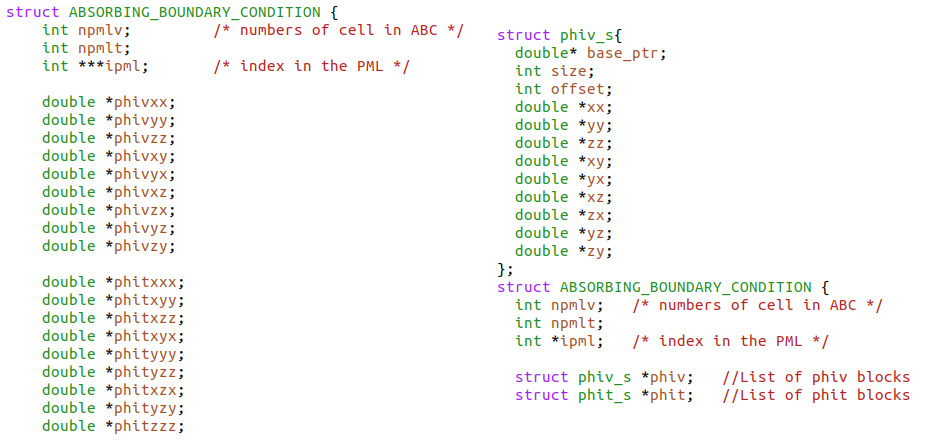
\includegraphics[width=35em]{abc}
    \end{center}
    \label{fig:abc}
    \legend{Fonte: Autor}
\end{figure}

A Figura \ref{fig:compute_address} mostra uma \textit{macro} desenvolvida para simplificar o acesso aos vetores utilizando a estrutura
descrita, onde o acesso a cada uma das componentes é dado calculando a soma do endereço base com o deslocamento associado ao vetor desejado.

\begin{figure}[!htb]
  \caption{\textit{Macro} desenvolvida para construir a nova estrutura proposta.}
    \begin{center} 
      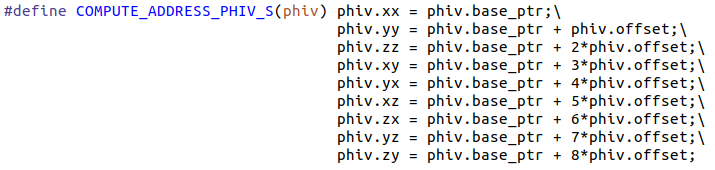
\includegraphics[width=35em]{compute_address}
    \end{center}
    \label{fig:compute_address}
    \legend{Fonte: Autor}
\end{figure}

Finalmente, na estrutura \textit{ABSORBING\_BOUNDARY\_CONDITION}, os conjuntos de vetores $phiv$ e $phit$ foram substituídos por vetores
dos tipos \textit{phiv\_t} e \textit{phit\_t}, com tamanho igual ao número de blocos do problema. Dessa forma, sendo $lx$ a quantidade
de blocos de cada linha do domínio, cada bloco ($i$, $j$) encontra em $phiv\_t[lx * i + j]$ o conjunto de vetores associados
às contribuições das bordas em ($i$, $j$).

Esse particionamento realizado introduziu a necessidade de adaptar o vetor $ipml$, responsável por associar cada coordenada à sua posição
nos vetores $phiv$ e $phit$. Anteriormente, o valor armazenado era um índice global, utilizado em vetores que representavam o domínio
completo do problema. Com a nova estrutura, é necessário que esses índices sejam locais, associados aos vetores que pertencem à um bloco
cada um.

Implementando todas as modificações descritas acima, o particionamento dos vetores das condições de borda proposto permite que cada
tarefa acesse apenas as posições que lhe são necessárias e o paralelismo entre blocos se torna possível.

\subsection{Criação de \textit{data handles}}

Para que os dados sejam acessados pelas tarefas submetidas na forma de \textit{buffers}, foi necessário encapsulá-los em
\textit{data handles} implementados pela biblioteca \textit{StarPU} e responsáveis por gerenciar réplicas dos dados envolvidos.
Durante a execução desse projeto foram utilizadas as funções \textit{starpu\_data\_vector\_register},
\textit{starpu\_data\_matrix\_register} e \textit{starpu\_data\_block\_register} para encapsular vetores unidimensionais,
matrizes e tensores tridimensionais, respectivamente. Essas funções têm como argumentos o endereço de início e as dimensões dos
dados, valores que posteriormente são acessíveis dentro das tarefas.

A biblioteca \textit{StarPU} oferece funções para realizar o ladrilhamento dos dados contidos em seus \textit{data handles} através
de filtros chamados \textit{starpu\_data\_filter}, que têm como parâmetros o número de blocos a serem criados e o ponteiro para uma
função que implementa o particionamento desejado.

No caso desse estudo, os blocos são formados no plano $XY$, mantendo cada um deles com uma altura igual à do domínio. Portanto, foi
necessário a aplicação de duas funções de particionamento, uma responsável pelo eixo $X$ e outra pelo eixo $Y$. Através da função
\textit{starpu\_data\_map\_filters}, foi possível executar o ladrilhamento de um conjunto de dados utilizando a composição de
diferentes funções de particionamento.

Depois de aplicar o filtro nos dados desejados, o acesso aos blocos é realizado através da função \textit{starpu\_data\_get\_sub\_data},
que tem como argumentos o \textit{data handle} original, o número de dimensões no qual ele foi particionado e os índices do bloco em cada
uma dessas dimensões. Dessa maneira é possível fornecer para cada tarefa apenas os bloco que lhe são necessários.

Finalizados os cálculos, os dados dos \textit{data handles} podem ser recuperados em suas estruturas originais após
uma chamada à função \textit{starpu\_data\_unregister}. A Figura \ref{fig:data_cycle} resume o ciclo de vida de uma dessas estruturas ao
longo da implementação desenvolvida.

\begin{figure}[!htb]
  \caption{Ciclo de vida de um \textit{data handle}.}
    \begin{center} 
      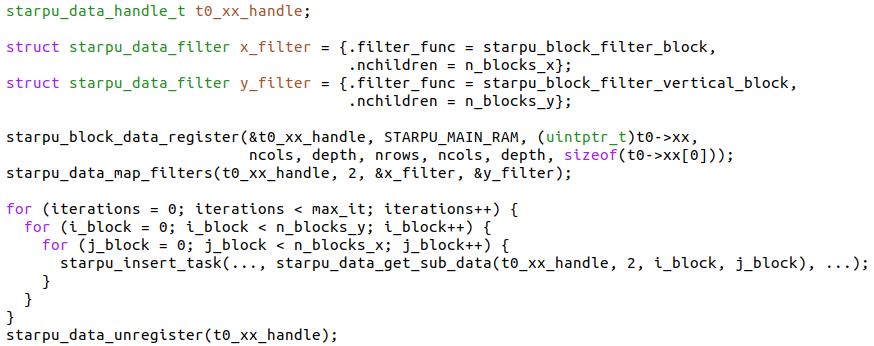
\includegraphics[width=35em]{data_cycle}
    \end{center}
    \label{fig:data_cycle}
    \legend{Fonte: Autor}
\end{figure}

\subsubsection{Acesso aos vizinhos}\label{sec:neighborhood}

Sendo o \textit{Ondes3D} um \textit{stencil}, a aplicação de um ladrilhamento implica em uma dificuldade introduzida na gestão de seus
vizinhos, pois o cálculo dos elementos posicionados nas bordas de um bloco necessita de dados presentes em outros blocos. Para solucionar
esse problema mantendo o particionamento, é necessário que cada tarefa receba não só o bloco do tensor a ser atualizado mas também blocos
dos tensores lidos nas posições vizinhas. É importante ressaltar que os vizinhos são acessados em modo de leitura, permitindo
que o paralelismo entre as tarefas de uma mesma etapa seja mantido.

No caso da implementação proposta, onde o ladrilhamento ocorre apenas no plano $XY$, um bloco pode possuir de dois a quatro vizinhos
em função de sua posição no domínio: blocos posicionados em um dos quatro cantos do plano $XY$ possuem apenas dois vizinhos, enquanto
os demais blocos posicionados nas bordas possuem três e os internos possuem quatro. Por isso, o laço de inserção de tarefas precisa
avaliar a posição tratada para construir um vetor de blocos contendo os vizinhos que serão utilizados em cada chamada.

No entanto, a implementação das tarefas tornou-se muito complexa ao utilizar essa solução. O cálculo realizado em cada célula ($i$, $j$, $k$)
não depende apenas de seus quatro vizinhos diretos, mas também dos quatro vizinhos posicionados a duas células de distância. Desde que o tamanho
do bloco seja maior que dois, essa propriedade não interfere na gestão dos vizinhos em si. Porém, dentro de cada tarefa, torna-se
necessário tratar uma quantidade significativa de casos distintos. São eles:

\begin{itemize}
\item{Células na primeira ou última linha do bloco:} índices do tipo $i - 1$ e $i - 2$ acessam os blocos vizinhos enquanto índices do tipo $i$ acessam o bloco principal 
\item{Células na primeira ou última coluna do bloco:} índices do tipo $j - 1$ e $j - 2$ acessam os blocos vizinhos enquanto índices do tipo $j$ acessam o bloco principal
\item{Células na segunda ou penúltima linha do bloco:} índices do tipo $i - 2$ acessam os blocos vizinhos enquanto índices do tipo $i$ e $i - 1$ acessam o bloco principal
\item{Células na segunda ou penúltima coluna do bloco:} índices do tipo $j - 2$ acessam os blocos vizinhos enquanto índices do tipo $j$ e $j - 1$ acessam o bloco principal
\item{Demais células:} todos os índices acessam o bloco principal
\end{itemize}

Além das possibilidades listadas, as operações realizadas são implementadas em funções que acessam mais de uma célula, criando assim
ainda mais situações possíveis a serem consideradas. A Figura \ref{fig:neighborhood} ilustra os acessos necessários para parte do cálculo
da célula ($i$, $j$) do bloco ($l$, $k$) do tensor de velocidade na direção do eixo $z$ na etapa \textit{computeVelocity}.

\begin{figure}[!htb]
  \caption{Parte do cálculo de $v0->z[i][j][k]$.}
    \begin{center} 
      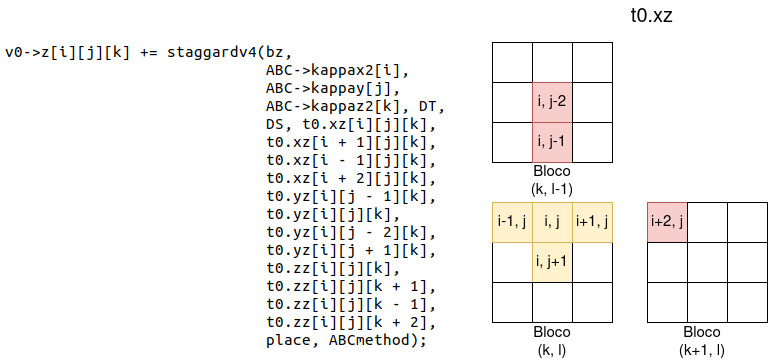
\includegraphics[width=32em]{neighborhood}
    \end{center}
    \label{fig:neighborhood}
    \legend{Fonte: Autor}
\end{figure}

Mesmo sendo mais eficiente em memória, o emprego da técnica de células fantasma, explicado na seção \ref{sec:proposal}, não diminui
a complexidade envolvida nesses casos. No entanto, constatou-se que os tensores cujos cálculos podem necessitar de blocos vizinhos não são
aqueles que estão sendo atualizados. No exemplo mostrado acima, são os valores de tensão que são consultados para calcular a velocidade
em uma dada coordenada. Sendo assim, optou-se por fornecer para cada tarefa um bloco, no caso dos dados que serão escritos, e o tensor
completo, no caso dos dados que serão lidos. Com isso, o paralelismo pode ser mantido, já que as escritas acontecem em dados independentes,
sem a necessidade de gerenciar leituras em blocos vizinhos.

Em contrapartida, conforme descrito anteriormente, um \textit{data handle} particionado não pode mais ser acessado da maneira original. Para isso, é necessário
utilizar a função \textit{starpu\_data\_unpartition}, que desfaz a operação de ladrilhamento anteriormente realizada. Essa operação exige a criação de um ponto
de sincronismo entre as tarefas para garantir que o \textit{data handle} foi reconstruído a partir de seus blocos atualizados na iteração atual, resultando na
criação de uma dependência que impossibilita que tarefas de duas etapas entre as quais exista essa reconstrução sejam executadas simultaneamente.

\subsection{Transformação em tarefas}\label{sec:task}

Cada um dos quatro \textit{macro-kernels} foi escrito seguindo a interface de tarefas \textit{StarPU}. Inicialmente serão abordados
os aspectos gerais dessa transformação, comuns a todas as etapas do algoritmo. Em seguida, a implementação da tarefa responsável
pelo cálculo da velocidade será vista em detalhes devido à particularidades nela encontradas.

A implementação de uma tarefa \textit{StarPU} começa pela leitura dos blocos utilizados, fornecidos na forma de \textit{buffers}, através 
das \textit{macros STARPU\_VECTOR\_GET\_PTR}, \textit{STARPU\_MATRIX\_GET\_PTR} e \textit{STARPU\_BLOCK\_GET\_PTR}. Além disso, é
necessário consultar as dimensões desses \textit{buffers}; apesar do ladrilhamento separar o espaço em blocos de tamanho igual, é possível
que as extremidades possuam blocos de tamanho menor caso não seja possível realizar uma divisão inteira.

Os laços internos, que originalmente percorriam uma região especificada na chamada do \textit{macro-kernel}, passam a percorrer o
tamanho de um bloco. No entanto, ao acessar as estruturas fornecidas apenas para leitura, é necessário realizar uma conversão das
coordenadas locais em coordenadas globais, já que elas não serão particionadas. A relação entre as coordenadas globais e locais é dada
pelas seguintes equações, onde $block\_size$ é o tamanho do bloco (aqui considerado quadrado), $i_{block}$ é o índice do bloco no eixo $x$
e $j_{block}$ é o índice do bloco no eixo $y$:

\[ i_{global} = block\_size * i_{block} + i_{local} \]
\[ j_{global} = block\_size * j_{block} + j_{local} \]


Para percorrer os vetores que eram originalmente acessados por suas coordenadas, três \textit{macros} foram implementadas em função
de suas dimensionalidades, conforme mostra a Figura \ref{fig:access}. Logo, todos os acessos à vetores foram substituídos por
chamadas às novas \textit{macros}.

\begin{figure}[!htb]
  \caption{\textit{Macros} utilizadas para acessar vetores.}
    \begin{center} 
      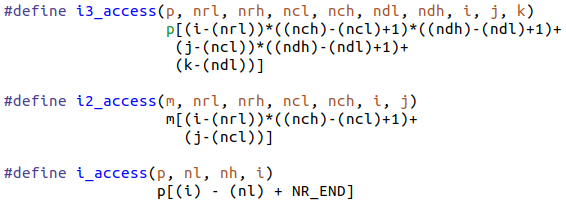
\includegraphics[width=34em]{access}
    \end{center}
    \label{fig:access}
    \legend{Fonte: Autor}
\end{figure}

\subsubsection{Cálculo de velocidades}
Apesar da seção \ref{sec:neighborhood} mostrar que cada uma das etapas só precisa acessar blocos vizinhos de estruturas em modo somente leitura, existe
uma exceção no cálculo de velocidade. Quando o índice $k$ é igual a $1$ ou $2$, certas operações adicionais são necessárias e estas
eventualmente envolvem blocos vizinhos onde outras tarefas precisam atualizar dados. No caso em que $k$ é igual a um, lê-se dados
do bloco seguinte no eixo $X$ e do bloco anterior no eixo $Y$, enquanto no caso em que $k$ é igual a dois, os dados externos pertencem
ao bloco anterior no eixo $X$ e posterior no eixo $Y$. 

Além da gestão dos vizinhos, a necessidade de consultar dados da mesma estrutura em que se está escrevendo adiciona também novas
dependências relativas à ordem dos cálculos. Se na aplicação original os vizinhos lidos são sempre aqueles cujas células já
foram atualizadas, é preciso manter essa mesma ordem na implementação paralela, quando cada bloco efetua seus cálculos independentemente.

O primeiro ponto demonstrado sugere que uma implementação de tarefas incluindo os possíveis vizinhos dos tensores de velocidade
seria capaz de resolver a questão, mas o segundo ponto mostra que só isso não é suficiente para garantir que o mesmo cálculo será
realizado. Por isso, a solução encontrada foi particionar a etapa de computação de velocidades em três \textit{kernels} diferentes, sendo
o primeiro deles responsável pelas células de índice $k$ igual a um, o segundo pelas células de índice $k$ igual a dois e o terceiro pelos
demais índices.

Em relação à vizinhança, em cada um dos casos especiais apenas um par de tensores de velocidade precisa de seus vizinhos, que conforme
descrito anteriormente, são no máximo dois blocos. Considerando essas particularidades, foi possível implementar essas tarefas de
maneira que os \textit{kernels} responsáveis pelos casos especiais tenham, cada um deles, apenas dois blocos vizinhos, que são fornecidos
apenas para leitura. A Figura \ref{fig:kernels_velo} apresenta um resumo da estrutura dessa etapa, onde a ordem de submissão das três
tarefas garante a ordem de execução necessária.

\begin{figure}[!htb]
  \caption{Resumo das chamadas de computação de velocidade.}
    \begin{center} 
      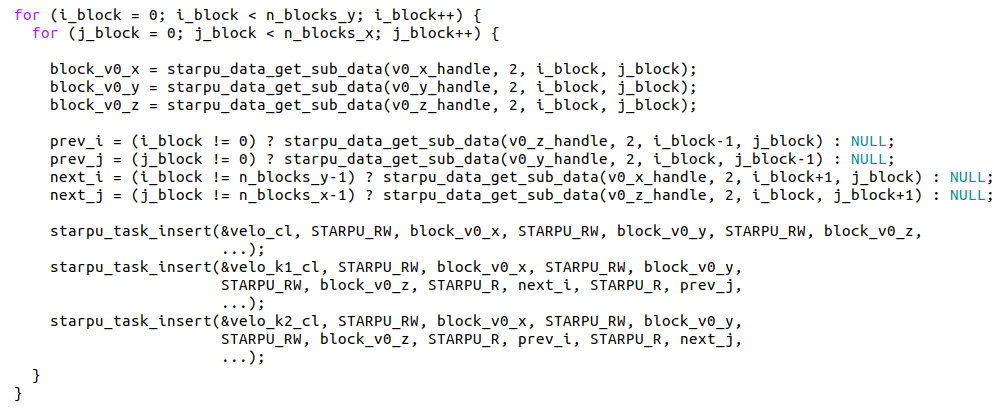
\includegraphics[width=35em]{kernels_velo}
    \end{center}
    \label{fig:kernels_velo}
    \legend{Fonte: Autor}
\end{figure}


\chapter{Avaliação experimental}

A nova versão desenvolvida foi executada no Parque Computacional de Alto Desempenho (PCAD) da Universidade Federal do Rio Grande do Sul com o
intuito de comparar seu desempenho em relação à implementação original.

\section{Ambiente de testes}
 // usar tambem cei e blaise
Para a execução dos testes, foram utilizadas as máquinas \textit{tupi} do PCAD, contando com um processador \textit{Intel Xeon E5-2620} com $8$
núcleos, $80$GB de memória RAM DDR$4$.
\section{Resultados}

Apesar do objetivo original ser a comparação da nova implementação com a antiga, não foi possível concluir o desenvolvimento da nova versão utilizando
a programação baseada em tarefas. Todas as tarefas foram construídas e o algoritmo é executado do início ao fim sem produzir erros de execução. No entanto,
ao comparar o resultado final obtido, não encontra-se o valor fornecido pela aplicação original.

Diversas investigações foram realizadas e indicam que os erros matemáticos encontram-se no cálculo das contribuições das condições de borda, etapa previamente
identificada como mais complexa. Devido ao tempo disponível, optou-se por apresentar o estudo desse desenvolvimento independentemente da corretude numérica dos resultados
devido ao valor científico das ponderações realizadas ao longo da implementação e também da possibilidade de realizar uma análise sobre o paralelismo alcançado
com as tarefas da maneira proposta.

** analise do paralelismo quando rolar o starvz **

\chapter{Conclusão}

relembra o contexto
digo o que fiz
quais foram os resultados
obstaculos

A sequência natural do trabalho apresentado é a correção dos erros numéricos introduzidos na mudança de modelo de programação realizada. Assim que esses resultados
forem alcançados, diversas melhorias podem ser postas em prática de maneira a acelerar ainda mais a execução da aplicação. Algumas delas são listadas abaixo:

\begin{itemize}
\item{Implementação visando arquiteturas heterogêneas:} assim como o trabalho desenvolvido por Martínez et al. \cite{victor}, é possível implementar \textit{kernels}
  que permitem a execução de tarefas em \textit{GPU}s.
\item{Implementação incluindo otimizações de operações de entrada e saída:} baseando-se nas alterações propostas por Boito et al. \cite{boito}, é possível construir uma versão
  paralela com uma quantidade reduzida de operações de entrada e saída, combinando os ganhos em eficiência de ambas as propostas.
%\item{Implementação visando paralelismo entre iterações:} duplicando as estruturas de dados, é possível manter em memória valores de duas iterações simultaneamente, o que
%  eventualmente possibilitaria uma execução que dispensa a necessidade de barreiras de sincronização entre iterações.
\item{Implementação de blocos de formato diferente:} em vez de limitar o ladrilhamento ao plano $XY$, a opção de particionar o espaço em todos os eixos permite o
  emprego de mais parâmetros que, refinados, podem gerar melhores resultados.
\item{Implementação de tarefas de granularidade menor:} as tarefas implementadas são compostas por diversas etapas menores, frequentemente associadas às diferentes
  regiões do domínio calculado. A transformação dessas etapas menores em tarefas resulta numa granularidade mais fina, o que pode contribuir para o equilíbrio de carga
  entre as unidades de execução.
\item{Refatoração do problema:} atualmente, a aplicação conta com uma função para cada grande etapa, resultando em longas implementações que tratam os mais diversos casos.
  Uma refatoração do código separando, por exemplo, o tratamento de cada região diferente, poderia não só facilitar o entendimento do algoritmo mas também permitir uma
  granularidade ainda mais fina na elaboração das tarefas.
\end{itemize}

% e aqui vai a parte principal
% 
% \chapter{Estado da arte}
% \chapter{Mais estado da arte}
% \chapter{A minha contribuição}
% \chapter{Prova de que a minha contribuição é válida}
% \chapter{Conclusão}

tupi pequena
cei media
blaise grande
% referências
% aqui será usado o environment padrao `thebibliography'; porém, sugere-se
% seriamente o uso de BibTeX e do estilo abnt.bst (veja na página do
% UTUG)
% 
% observe também o estilo meio estranho de alguns labels; isso é
% devido ao uso do pacote `natbib', que permite fazer citações de
% autores, ano, e diversas combinações desses

\bibliographystyle{abntex2-alf}
\bibliography{biblio}

\end{document}
